\clearpage
\section{A uniform remainder over all periods}\label{sec:uniform-period}
The previous section first derives the exact coefficient with a fixed cyclic inverse. We now control that inverse in a norm independent of the period and retain averaged phase errors. This strengthens the same local law, rather than asserting a finite-condition-number formula for the maximizing factor.

% R02 bounded investigation: uniformity over all finite binary words.
% Proof audit artifact only; do not edit a frozen manuscript.
\begin{theorem}[A remainder uniform over all finite BB words]
\label{thm:r02-uniform-cubic}
For every finite binary periodic word
$\bm\sigma=(\sigma_0,\ldots,\sigma_{L-1})$, $L\ge1$, let $(a_j)$ be
the unique periodic solution of
\[
 a_{j+1}-a_j+2a_{j-1}=2\sigma_j,
 \qquad q_j=\sigma_j-a_{j-1},
 \qquad K_{\bm\sigma}=\frac1{2L}\sum_jq_j^2.
\]
For every $0<C\le1/4$ and either
$Q_{\bm\sigma}=\Gamma_{\bm\sigma}$ or
$Q_{\bm\sigma}=q^{\rm fd}_{\bm\sigma}$,
\[
 \left|C-Q_{\bm\sigma}-K_{\bm\sigma}C^3\right|
 \le6400C^4.
\]
The constant is independent of the word, its length, and its minimal
period. Thus the word may depend on $C$. The same conclusion holds for
$q^{\rm H}_{\bm\sigma}$ and $\Theta^{\rm fd}_{\bm\sigma}$ by their
established identities with $\Gamma_{\bm\sigma}$.
\end{theorem}

\begin{proof}
All sequence norms below are normalized:
$\|v\|_{1,L}=L^{-1}\sum_j|v_j|$ and
$\|v\|_\infty=\max_j|v_j|$.
Write $(Sv)_j=v_{j+1}$ and $B=S-I+2S^{-1}$.
Put
\[
 \alpha=\frac{1+i\sqrt7}{4},\qquad
 h_k=\frac2{\sqrt7}\operatorname{Im}(\alpha^k),\quad k\ge1.
\]
The power series
\[
 H(z)=\frac{z}{z^2-z+2}=\sum_{k\ge1}h_kz^k
\]
converges absolutely on the unit circle and obeys
$H(S)B=BH(S)=I$ for every cyclic shift $S$. Moreover,
\[
 \sum_{k\ge1}|h_k|
 \le\frac{2(1+\sqrt2)}{\sqrt7}<2.
\]
Consequently $B^{-1}$ has operator norm at most $2$ both in
$\|\cdot\|_{1,L}$ and in $\|\cdot\|_\infty$, independently of $L$.
Since $B$ maps a constant to twice that constant,
\[
 a-\frac12=2B^{-1}\left(\bm\sigma-\frac12\right),\qquad
 \left\|a-\frac12\right\|_\infty\le2,\qquad
 \|q\|_\infty\le\frac52,\qquad
 \frac1L\sum_jq_j=0.
\]
In particular $V:=2K_{\bm\sigma}=L^{-1}\sum q_j^2\le25/4$.

Let $t=\operatorname{arctanh}C$ and $r_j=1+q_j$.
The established endpoint trajectory has factor $\rho_{\bm\sigma}>0$ and
\[
 g_{\rm ep}:=\log\frac C{\rho_{\bm\sigma}}
 =\frac1L\sum_j\log\cosh(tr_j)-\log\cosh t.
\]
Convexity, the mean identity $L^{-1}\sum r_j=1$, and the bound
$(\log\cosh)''\le1$ show
\[
 0\le g_{\rm ep}\le\frac V2t^2\le4C^2.
\]
Here $t\le(16/15)C$ for $C\le1/4$.
The elementary estimate
$|\log\cosh x-x^2/2|\le x^4/12$, together with
$|r_j|\le7/2$, yields
\[
 |g_{\rm ep}-K_{\bm\sigma}C^2|
 \le20C^4.                                             \tag{U1}
\]
For an explicit check of this last constant, one may use
$t-C\le16C^3/45$, $t+C\le31C/15$, and hence
\[
 \frac{(7/2)^4+1}{12}\left(\frac{16}{15}\right)^4
 +\frac{25}{8}\frac{496}{675}<20.
\]

Choose an ergodic maximizing invariant probability $\Pi$.
The endpoint lower bound ensures its logarithmic average is finite.
Let $r$ be its persistent active-hull contrast, and use the normalized
variables $x\in[-1,1]$, $\mu(w)=\int x\,dw$,
$J(w)=1-\int x^2\,dw$, and selector deviation $s$.
Set
\[
 G=\log(C/\Gamma_{\bm\sigma}),\qquad
 \Delta=\log(r/\Gamma_{\bm\sigma}).
\]
The endpoint-band and endpoint-trajectory bounds give
\[
 0\le\Delta\le G\le g_{\rm ep}\le4C^2,\qquad
 0\le C-r\le CG\le4C^3.                              \tag{U2}
\]
All expectations without a phase subscript refer to $\Pi$.

The endpoint defect, selector formulas, and stationarity give
\[
 \mathbb E s^2\le\frac{2\Delta}{(1-C)^2}\le16C^2,
 \qquad
 \mathbb E\mu^2
 \le2\mathbb E s^2+\frac{2r^2}{(1-r)^2}\le36C^2.       \tag{U3}
\]
Indeed, the BB2 selector differs from $\mu$ by at most $r/(1-r)$,
and the current and lag spectral marginals agree.
For $Z=\int(x-s)^2\,dw=1-J-2s\mu+s^2>0$,
\[
 f-\log r
 \le-\frac12J-s\mu+\frac12s^2+\frac r{1-r}|s|.
\]
Averaging gives
\[
 \mathbb EJ
 \le2\Delta+2\sqrt{\mathbb Es^2\,\mathbb E\mu^2}
       +\mathbb Es^2+\frac{2r}{1-r}\sqrt{\mathbb Es^2}
 \le84C^2.                                           \tag{U4}
\]
These are global invariant-measure bounds; no individual phase is
bounded by multiplying by $L$.

The uniform mean-update estimate established in the exact-coefficient
proof is
\[
 |\mu(w')-\mu(w)+2s|\le8(J+\mu^2)+12s^2.
\]
For completeness, its numerator before division by $Z$ is
$(m_3-\mu)+\mu J+2s\mu^2-4s^2\mu+2s^3$.
Using $|m_3-\mu|\le J$, the case $Z\ge1/2$ is immediate.
If $Z<1/2$, then $J+\mu^2>1/2$ from
$Z=1-J-\mu^2+(s-\mu)^2$, and the trivial bound on the left is $4$.
Thus no lower bound on $Z$ is assumed.

Let $\Pi_j$ be the normalized phase-$j$ conditional law, and set
$M_j=\mathbb E_{\Pi_j}\mu(w)$ and $S_j=\mathbb E_{\Pi_j}s$.
The exact phase equations can be written
\[
 M_{j+1}=M_j-2S_j+e_j,\qquad
 S_j=M_{j-1}+r\sigma_j+\eta_j .
\]
Uniform phase probabilities and (U3)--(U4) yield
\[
 \|e\|_{1,L}\le8(84+36)C^2+12(16)C^2=1152C^2.        \tag{U5}
\]
For BB2,
\[
 s_1(w)-\mu(w)-r
 =-\frac{r(J(w)+\mu(w)^2+r\mu(w))}{1+r\mu(w)}.
\]
BB1 has zero selector remainder. Therefore
\[
 \|\eta\|_{1,L}
 \le\frac r{1-r}
      \left(\mathbb EJ+\mathbb E\mu^2+r\mathbb E|\mu|\right)
 \le168C^3.                                          \tag{U6}
\]
The lag at phase $j$ has the current law at phase $j-1$, which explains
both the index and the absence of any phase-count factor.

Combining the phase equations gives
\[
 BM=-2r\bm\sigma+e-2\eta,\qquad
 \|e-2\eta\|_{1,L}\le1236C^2.
\]
Since $Ba=2\bm\sigma$, the uniform inverse bound yields
\[
 \|M+ra\|_{1,L}\le2472C^2,\qquad
 \|S-rq\|_{1,L}\le2514C^2,\qquad
 \|S-Cq\|_{1,L}\le2517C^2.                            \tag{U7}
\]
The last inequality also uses (U2) and $\|q\|_\infty\le5/2$.

We do not need a bound on the mean square of the phase error.
The pointwise inequality $S_j^2\ge2Cq_jS_j-C^2q_j^2$ instead gives
\[
 \frac1L\sum_jS_j^2
 \ge VC^2-2C\|q\|_\infty\|S-Cq\|_{1,L}
 \ge VC^2-12585C^3.
\]
Conditional Jensen and the endpoint defect imply
\[
 G\ge\Delta\ge\frac{(1-C)^2}{2L}\sum_jS_j^2
 \ge K_{\bm\sigma}C^2-6300C^3.                        \tag{U8}
\]
In the last step, $V\le25/4$ and
$25/4+12585/2<6300$ suffice.
By (U1)--(U2),
\[
 |G-K_{\bm\sigma}C^2|\le6300C^3.
\]
Since $0\le G\le4C^2$ and
$|1-e^{-G}-G|\le G^2/2$,
\[
 |C-\Gamma_{\bm\sigma}-K_{\bm\sigma}C^3|
 \le6302C^4.
\]
The endpoint factor itself satisfies
$|C-\rho_{\bm\sigma}-K_{\bm\sigma}C^3|\le28C^5\le7C^4$.
The established sandwich
$\rho_{\bm\sigma}\le q^{\rm fd}_{\bm\sigma}
 \le\Gamma_{\bm\sigma}$
therefore proves the advertised constant $6400$ for both factors.
Constant words have $q_j=0$ and exact factor $C$, consistently with
the statement.
\end{proof}

\begin{corollary}[Growing equal blocks]
\label{cor:r02-growing-blocks}
Let $\bm\sigma^{(m)}=0^m1^m$ and put $\theta=2^{-1/2}$. Then
\[
 \left|K_{\bm\sigma^{(m)}}-\frac3{16m}\right|
 \le\frac4{7m}\frac{\theta^m}{1-\theta^m}.             \tag{U9}
\]
Consequently, if $C\downarrow0$, $m=m(C)\to\infty$, and $mC\to0$,
then for $Q=\Gamma$ or $q^{\rm fd}$,
\[
 C-Q_{\bm\sigma^{(m)}}(C)
 =\frac{3C^3}{16m}
   \left[1+O(\theta^m)+O(mC)\right]
 \sim\frac{3C^3}{16m}.
\]
The condition $m\to\infty$ is essential for replacing the exact
coefficient by $3/(16m)$.
\end{corollary}

\begin{proof}
From $q=\bm\sigma-S^{-1}a$ and $a=2B^{-1}\bm\sigma$,
\[
 q=B^{-1}(S-I)\bm\sigma.
\]
For $0^m1^m$, the cyclic difference has two opposite unit impulses
separated by $m$. Let
\[
 R(d)=\sum_{k\ge1}h_kh_{k+d}\quad(d\ge0).
\]
Absolute convergence permits all rearrangements. Direct geometric
summation gives
\[
 R(0)=\sum_{k\ge1}h_k^2=\frac38,\qquad
 |R(d)|\le\frac47\theta^d.
\]
For example,
$R(0)=\frac27[1-\operatorname{Re}(\alpha^2/(1-\alpha^2))]$ and
$\operatorname{Re}(\alpha^2/(1-\alpha^2))=-5/16$.
Periodizing the impulse response over $2m$ and expanding its squared
norm gives
\[
 \sum_{j=0}^{2m-1}q_j^2
 =2R(0)+4\sum_{n\ge1}(-1)^nR(nm).
\]
Since $K=(4m)^{-1}\sum_jq_j^2$, the geometric tail bound proves (U9).
The uniform theorem contributes an absolute $O(C^4)$ error, or a
relative $O(mC)$ error after division by $3C^3/(16m)$.
\end{proof}


\begin{corollary}[A conservative analytic comparison certificate]
Let $\bm\sigma$ and $\bm\tau$ be finite binary words with
$K_{\bm\sigma}>K_{\bm\tau}$, and choose consistently either
$Q=\Gamma$ or $Q=q^{\rm fd}$. Then
\[
 Q_{\bm\sigma}(C)<Q_{\bm\tau}(C)
 \quad\hbox{if}\quad
 0<C<\min\left\{\frac14,
          \frac{K_{\bm\sigma}-K_{\bm\tau}}{12800}\right\}.
\]
Indeed,
$Q_{\bm\tau}-Q_{\bm\sigma}
 \ge (K_{\bm\sigma}-K_{\bm\tau})C^3-12800C^4$.
For example,
$K_{000111}-K_{001011}=1/21$, giving the sufficient range
$0<C<1/268800$.
This is a conservative comparison of asymptotic factors, not a
finite-iteration or finite-budget guarantee.
\end{corollary}


\begin{figure}[ht]
\centering
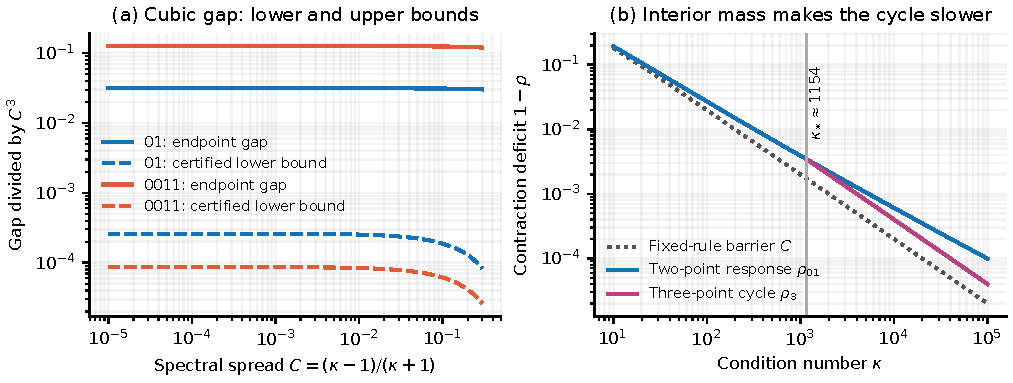
\includegraphics[width=.96\textwidth]{figures/mechanism.pdf}
\caption{Supporting exact-factor mechanisms. Left: the unrestricted gap lies between the conservative transition-frequency certificate and the endpoint gap. These are formula evaluations, not fitted unrestricted factors. Right: above $\kappa_*$ the three-point alternating cycle is slower than the endpoint response.}
\end{figure}

\paragraph{Scope of the numerical illustration.}
The main coefficient figure uses the 113 balanced primitive rotation classes among the 745 exact responses through length 12, together with the 64 recorded equal-block coefficients. Its left panel illustrates the proved density bounds and the two comparison phenomena; its right panel evaluates the exact coefficient formula. The companion \texttt{word\_figure/} directory includes the fixed inputs, generated tables, plotting program, and reproduction instructions. No new optimizer benchmark or empirical fit of $\Gamma$ enters the uniform theorem.
